\subsection{Argentina}\label{subsec:arg}
%\subsubsection{Bariloche}

The site in Bariloche is located at the Centro Atómico Bariloche, see table
\ref{tab:locations}. As mentioned in section \ref{sec:electronics} the
Bariloche group has developed the electronics for the LAGO project in
collaboration with the Mexico group. The detectors in this site are mostly used
to test and improve the data acquisition software and hardware since 2006. 
In addition, the use of these WCD were of outmost importance for the first
space wheather studies within the LAGO collaboration (see section
\ref{sec:science}).

%\subsubsection*{Detectors description}
Three different WCD have been assembled. Nahuelito was the first detector build in 2006
and together with Boyita are made of commercial plastic water tanks. Recently a
stainless steel commercial water tank has been used in the construction of
Sputnik. The latter will serve as a prototype for the Antarctic site detector
(section \ref{sec:antartica}). Geometry and dimensions details of these three
detectors are shown on figure \ref{fig:bar-tanques}.

\begin{figure}[h!]
\begin{center}
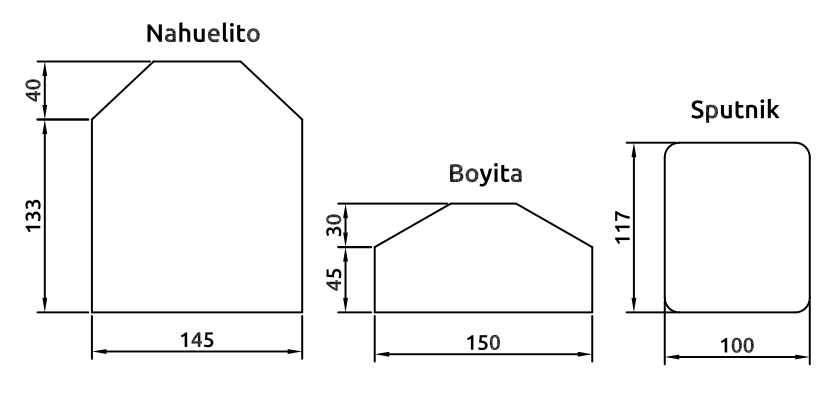
\includegraphics[width=0.8\textwidth]{images/argentina/tanques-bariloche.png}
\caption{Geometry and dimensions of the Bariloche site detectors (all units in cm).} 
\label{fig:bar-tanques}
\end{center}
\end{figure}

All detectors have an inner liner made of Tyvek$^{\textregistered}$ and one PMT mounted on top.
Both Nahuelito and Boyita have 8\,'' Hamamatsu R5912 PMTs while Sputnik has an
8\,'' Electron Tube Limited 9353KB PMT. Because of the good water quality of Bariloche
no purification process was implemented and tap water is used directly. The possibility of
doping the water with Amino-G (NH$_2$C$_{10}$H$_5$(SO$_3$H)SO$_3$Na) as wavelength shifter
to improve the signals has been explored in all the Bariloche detectors. 
 
%\subsubsection*{Detectors performance}

During the last years the use of the detectors has been shared with
experimental physics courses for Balseiro Institute undergraduate students.
Currently only Nahuelito is used exclusively for the LAGO project. In this
section different results are presented using the three detectors to showcase
their performance.

Muon decay can be observed using WCD by looking at the histogram of time
difference between consecutive events as shown on figure \ref{fig:bar-data},
left.  Two different regions can be seen. At large time differences the
exponential distribution corresponding to the arrival of uncorrelated particles
from the background of secondary cosmic rays. At small time differences another
exponential distribution with a characteristic time $\approx$2\,$\mu$s
corresponding to muon decay \cite{}.

Charge and amplitude histograms are used to calibrate the detectors. The
maximum of the muon hump, corresponding roughly to verticals muons, can be used
to define the VEM (Vertical Equivalent Muon). $1\,$VEM is the average signal of
a vertical and central muon. The final energy calibration of the detectors can
be done knowing the average energy deposited by a vertical muon. A typical
charge histogram of Boyita can be seen in figure \ref{fig:bar-data}, center.

During the construction of Sputnik the improvements on the signals due to the
inner Tyvek$^{\textregistered}$ liner and the addition of Amino-G to the water
was checked. Comparison of average signals taken with the stainless steel tank
only and the addition of the inner liner and Amino-G (6\,mg/l) can be seen in
figure \ref{fig:bar-data}, right. All the signals were taken using an oscilloscope
with a trigger rate of approximately 100\,Hz. Using the LAGO data acquisition
electronics with a sampling rate of 40\,MHz the charge-amplitude ratio goes
from 1 in the case of bare stainless steel to approximately 1.5 with the
addition of the Tyvek$^{\textregistered}$ liner and to approximately 2 doping
the water with Amino-G.  

\begin{figure}[h]
 \begin{center}
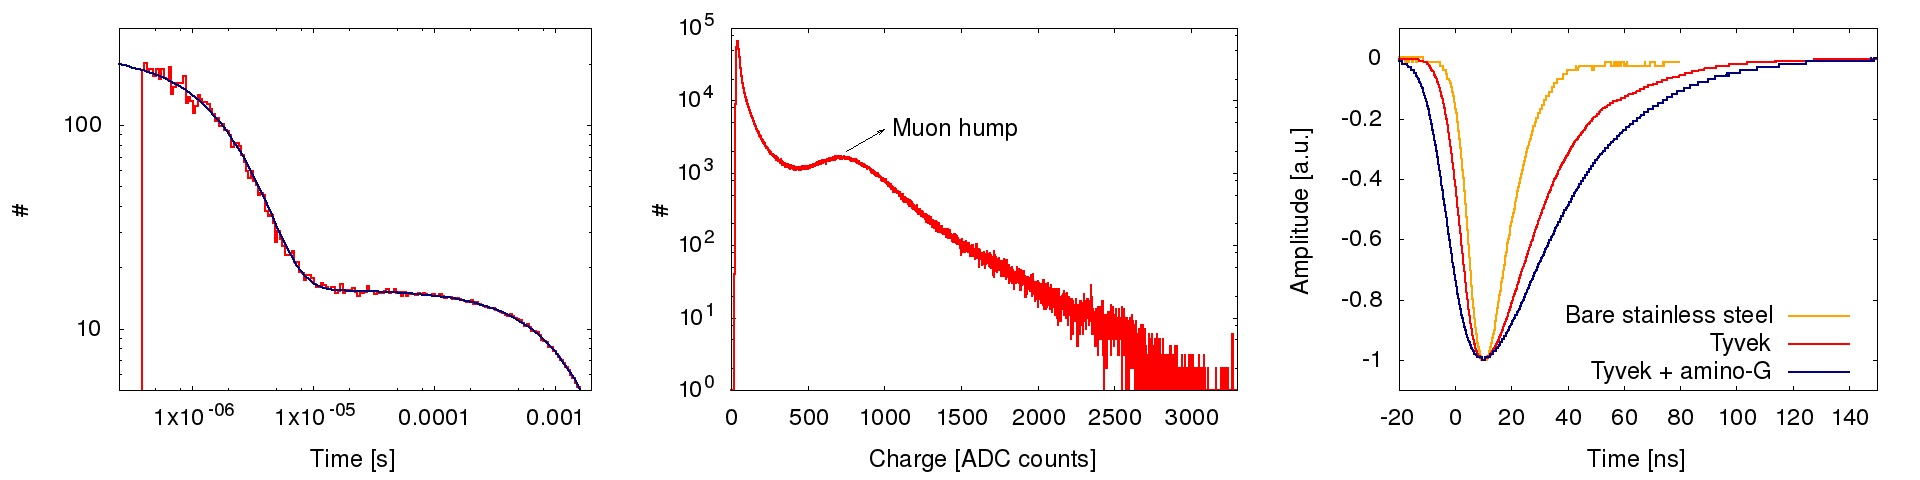
\includegraphics[width=\textwidth]{images/argentina/data.png} \caption{Left: histogram
of time difference between consecutive events using Nahuelito. A fit of the sum
of two exponential functions corresponding to muon decay and the arrival of
uncorrelated particles of the background can be observed. Center: one hour
typical charge histogram using Boyita. Right: Comparison of average traces with
the stainless steel tank only and after the addition of the
Tyvek$^{\textregistered}$ liner and Amino-G. A significant improvement of the signal
is observed.} \label{fig:bar-data} 
\end{center}
\end{figure}

The addition of Amino-G as wavelength shifter significantly improves the
signals of WCD. However a systematic study of the aging of Amino-G doped water would be
necessary before deciding on its use in all LAGO detectors.

%\subsubsection{Buenos Aires}

The detector located in Buenos Aires is at the campus of the Universidad de
Buenos Aires (UBA), in the building of the Instituto de Astronomía y Física del
Espacio (IAFE), se table \ref{tab:locations}. It is used mainly to test the
remote operation and low level of local maintenance requirements, for those
detectors requiring high levels of autonomy. This detector is used also to test
resistance to extreme conditions (e.g., extreme low temperatures).  The group
of Buenos Aires is the responsible of the project 'LAGO in Antartic' (see
Section \ref{sec:antartica}).

%\subsubsection*{Detector description}

\begin{figure}[h!]
\begin{center}
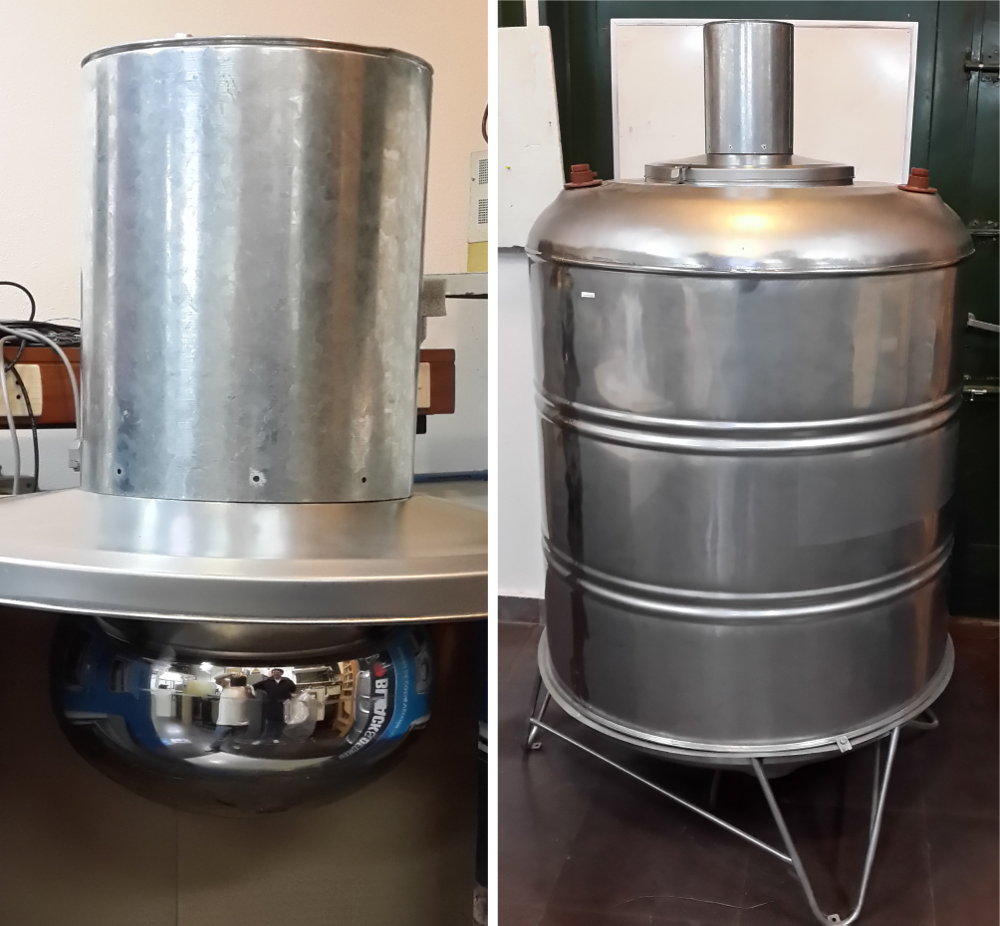
\includegraphics[width=0.8\textwidth]{images/argentina/neurus.png}
\caption{Neurus detector. Left: support for the PMT and its electronic base
(connectors are above [not shown]). Right: The detector with the base of the
PMT (isolated for humidity) above and outside the water container, inside the
tall top hat.}
\label{fig:neurus}
 \end{center}
\end{figure}

A WCD, labeled 'Neurus', was constructed and it is a prototype for the detector
to be installed at the first site of LAGO-Antartica.  The water container is a
stainless steel commercial water tank.  The geometry and dimensions of the
water container are the same as Sputnik detector at Bariloche (see right side
of Figure \ref{fig:bar-tanques}).  It has an inner liner made of
Tyvek$^{\textregistered}$ and one PMT of 9'' PHOTONIS XP1805 mounted on its top.
The water is purified using a standard commercial filter for human consuming,
removing the chlorine present in the water of the net.  In order to minimize
the presence of humidity in the electronic, the base of the PMT is isolated in
a tall top hat, outside the water recipient (see Figure \ref{fig:neurus}). At
the moment, Neurus is used exclusively for the LAGO project, and we plan to
share it in the near future for experimental undergraduate physics courses for
students from the physics department of the Universidad de Buenos Aires.

%\subsubsection{LAGO in Antartica}
\label{sec:antartica}

For developing scientific research associated with the branches of Space
Physics and Space Weather in LAGO (see section \ref{sec:science}), low values
for rigidities cut-off are desirable.  Sites located at low magnetic latitudes
are then favorable for installing new LAGO detectors. Antartica is then an
excellent place to this purpose.  In this section, we describe the project
'LAGO in Antartica', a project to install detectors inside the Argentina sector
of Antartica.

%\begin{figure}[h!]
%\begin{center}
%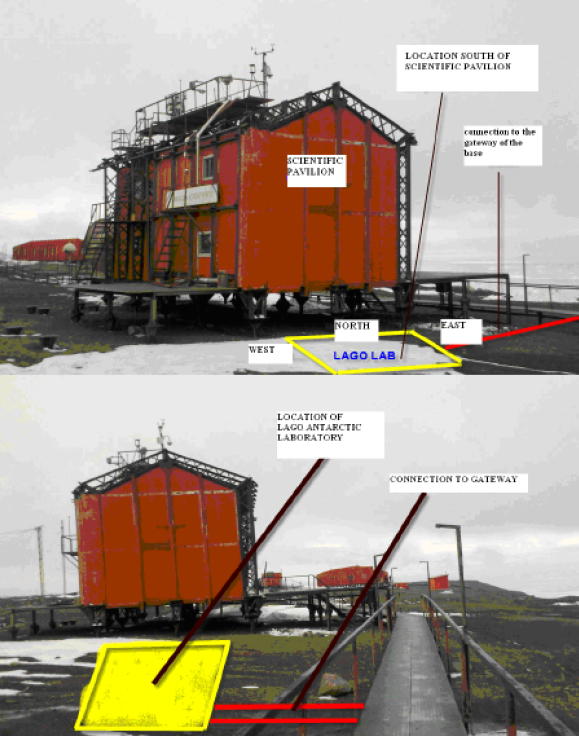
\includegraphics[width=0.8\textwidth]{images/argentina/site_labo_marambio.png}
%\caption{Location of the proposed LAGO node at
%Marambio Station .}
%\label{fig:marambio-location}
%\end{center}
%\end{figure}

The activities developed for selecting and planning the antartic site, as well
as for constructing the laboratory are included into a frame of collaboration
between the Instituto Ant\'artico Argentino (Direcci\'on Nacional del
Antartico, IAA/DNA), the Instituto de Astronomia y Fisica del Espacio (IAFE,
UBA-CONICET), and the LAGO network collaboration.

After our campaign during the austral summer of 2011 to determine the best site
location for the LAGO laboratory in Antartica, we concluded that due to the
possibilities of constructing a new building and due to the infrastructure
available, the Marambio base is the best option for locating the first
Antarctic LAGO node.

For safeguard and operational resources reasons, it was decided to mount the
module near the scientific pavilion. The new LAGO laboratory will be located
in such way that will be possible to access through by a gateway from/to the
already installed scientific pavilion. This is important because our study of
winds (intensities and directions) predict the existence of strong winds during
winter time and the idea is that the hard outside enviroment do not affect the
maintenance of the detectors. The following photos show the place on figure
\ref{fig:marambio-location}.

Due to the low temperatures at Marambio, the cherenkov detectors should be
protected at an over zero Celsius environment.  A laboratory to locate the
detectors is projected to be constructed. 
% The plan floor of the laboratory to
%be constructed is shown in Figure \ref{fig:planfloor}.

%\begin{figure}[h!] \begin{center}
%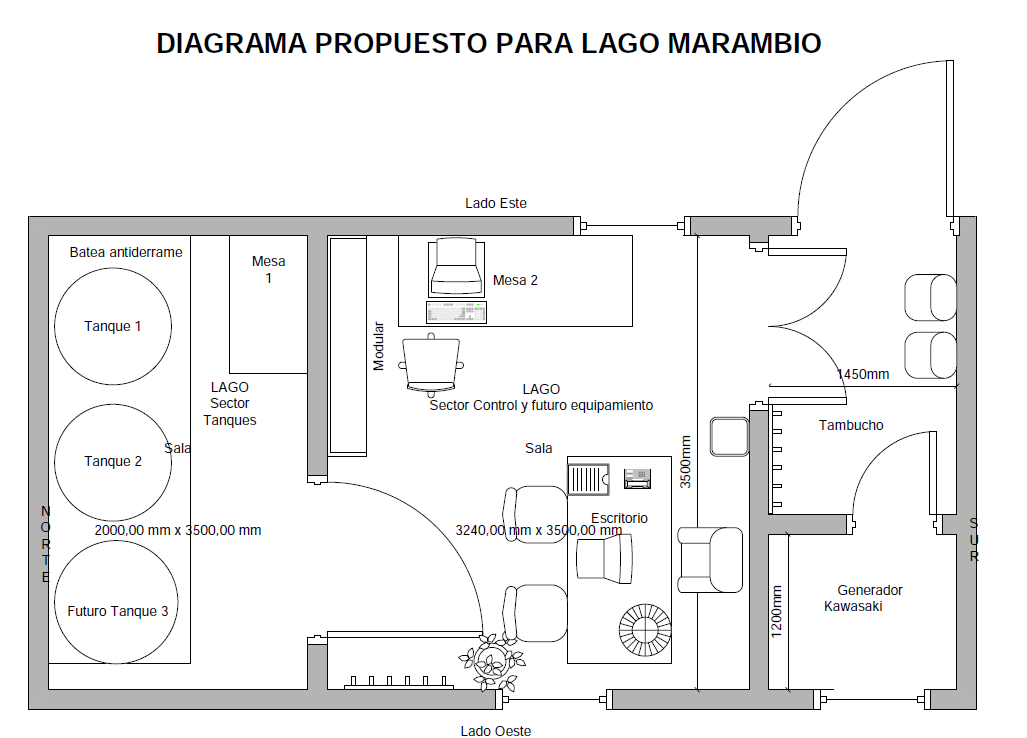
\includegraphics[width=0.8\textwidth]{images/argentina/plano_labo_marambio.png}
%\caption{Plan floor of the LAGO laboratory at Marambio .} \label{fig:planfloor}
%\end{center} \end{figure}

The election of this site is also supported from a series of numerical
simulations of different conditions for the arrival of cosmics rays at this
site.  The cutoff rigidity at Marambio, for quiet geomagnetic
conditions, is R$_c^{Mr}$ = (2.3 $\pm$ 0.2) GV \cite{Masias2014}.
It has a dependence with the geomagnetic activity and Marambio is magnetically
connected to the polar oval, consequently this site will be the first LAGO site
available to observe precipitation of particles from this region of the
magnetosphere.
Also, the study of the sensitivity of $R_c$ to geomagnetic storms at Marambio using
the Dst index as a proxy to quantify the strenght of the storm, finding a
relative rate of change of $\frac{1}{Rc}\frac{\Delta Rc}{\Delta
Dst}=3\times10^{-3}$nT$^{-1}$ \cite{Masias2014}. 
%$1/Rc (\Delta Rc / \Delta Dst)$ at BsAs is $-0.1/nT$, and at Marambio is
%$-0.3/nT$.
%This result can be seen in Figure \ref{fig:bsas_marambio}, where values for
%Buenos Aires are also included for comparison; 
%Changes in R$_c$ imply that lower rigidity particles can reach Earth during periods active of geomagnetic storms.

%%\begin{figure}[h!]
%%\begin{center}
%%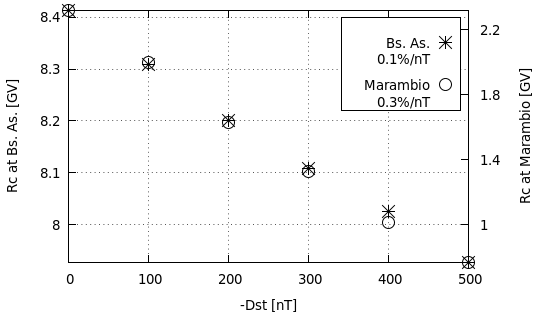
\includegraphics[width=0.8\textwidth]{images/argentina/dst_vs_Rc_bsas_and_marambio_LAGO.png}
%%\caption{Rigidity cut-off for different global geomagnetic activity (Dst index
%%used as proxy) for Buenos Aires and Marambio base in Antartica. Adapted from \cite{Masias2014}.}
%%\label{fig:bsas_marambio}
%%\end{center}
%%\end{figure}
%%
